\chapter{Results}
This results chapter is meant as a mechanism to present all of the data that was collected on the performance of different demodulator. All of the demodulators that were tested in the course of this research will be shown whether that be dedicated hardware or software. The first results that will be shows are those of the dedicated hardware, being TNCs and Argent Data's Open Trackers. Following the hardware will be the software implementations. And following that will be some general comparisons between the hardware and software.

\section{Dedicated Hardware Results}
Before presenting all of the data on how many packets were correctly demodulated in each one of the five test files, each one of the pieces of hardware will listed.  In the scope of this research a total of 12 pieces of hardware were tested and they are Argent Data's Open Tracker 2, Open Tracker 3, Open Tracker USB, Open Tracker 3 Micro, Kantronics Kam, two Kantronics Kam Plus, two AEA PK-88, a PK-232, a PK-232MBX, and an MFJ-1278. Please note that on the figures Open Tracker will be abbreviated OT.

The first two tests consisting of clean packets - 40 generated from the Open Tracker and 200 using Toledo's suite - was relatively uninteresting. Essentially every piece of hardware decoded all 40 and all 200 packets. The only anomalies to this were that the Open Tracker USB was only able to decode 39 and 193 out of the 40 and 200 packet files respectively. Additionally the Open Tracker 3 Micro missed one packet in the 200 packet file to only decode 199. For these since there is no real way to debug and see the cause of decoding relatively fewer or more packets just the data is presented as it was measured to allow for comparison to the software. This will continue to be the case for the remainder of this hardware section.

Following the two easy files the next file is same content as the file with 40 packets in it with the only difference being that noise was progressively added. In Figure \ref{allHardwareOT3Noise} the two PK-88s stand out for being able to decode 25 of the 40 packets in this file.

 \begin{figure}
  \centering
	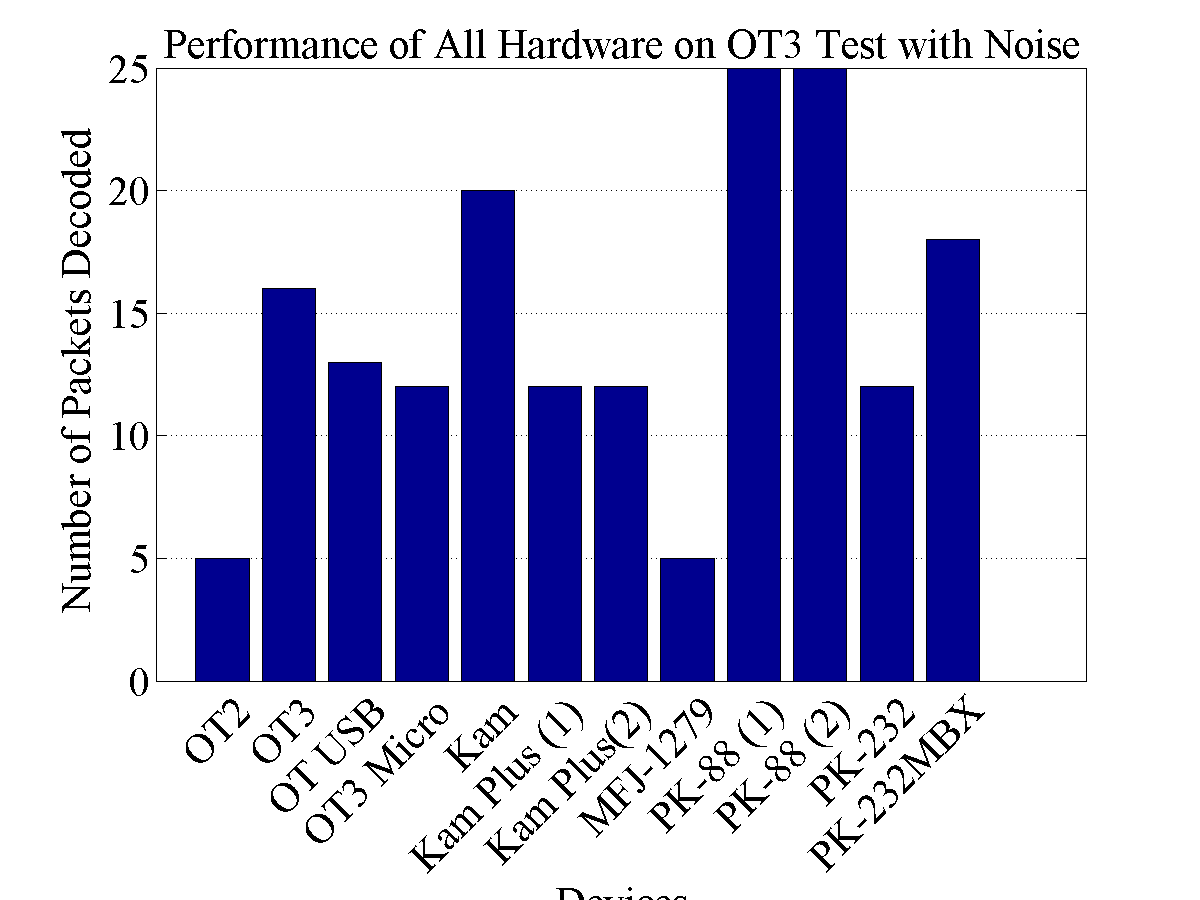
\includegraphics[width=0.75\linewidth]{images/PerformanceofAllHardwareonOT3TestwithNoise.png} 
	\caption{Number of packets successfully decoded for all tested hardware on Open Tracker 3 test file with noise.}
   \label{allHardwareOT3Noise}
\end{figure}

The next two files are the ones that were used most extensively in the testing for comparison and tuning. Primarily the first which is just a recording of traffic off the air. They are Track 1 and 2 from the APRS CD mentioned in the Demodulator Benchmarking Chapter. The results from Track 1 are in Figure \ref{allHardwareTrack1} and Track 2 in Figure \ref{allHardwareTrack2}. The top three of the hardware on Track 1 was the PK-88 (2) with 1007 packets decoded, the Kam with 988 Packets, and the Kam Plus (2) with 985 Packets. For Track 2 the top hardware was the Kam Plus (2) with 998, the Kam Plus (1) with 967, and the Kam with 938.

 \begin{figure}
  \centering
	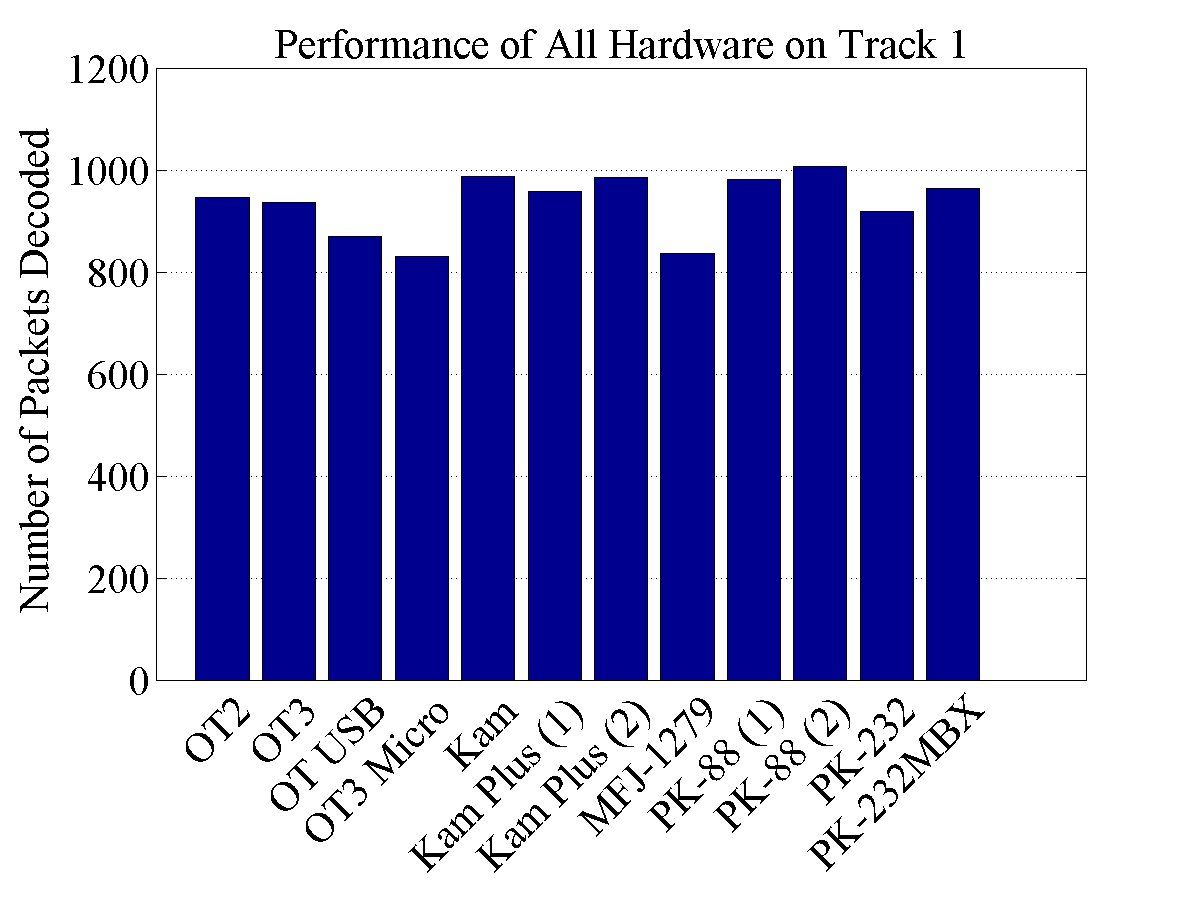
\includegraphics[width=0.75\linewidth]{images/PerformanceofAllHardwareonTrack1.png} 
	\caption{Number of packets successfully decoded for all tested hardware on Open Tracker 3 test file with noise.}
   \label{allHardwareTrack1}
\end{figure}

 \begin{figure}
  \centering
	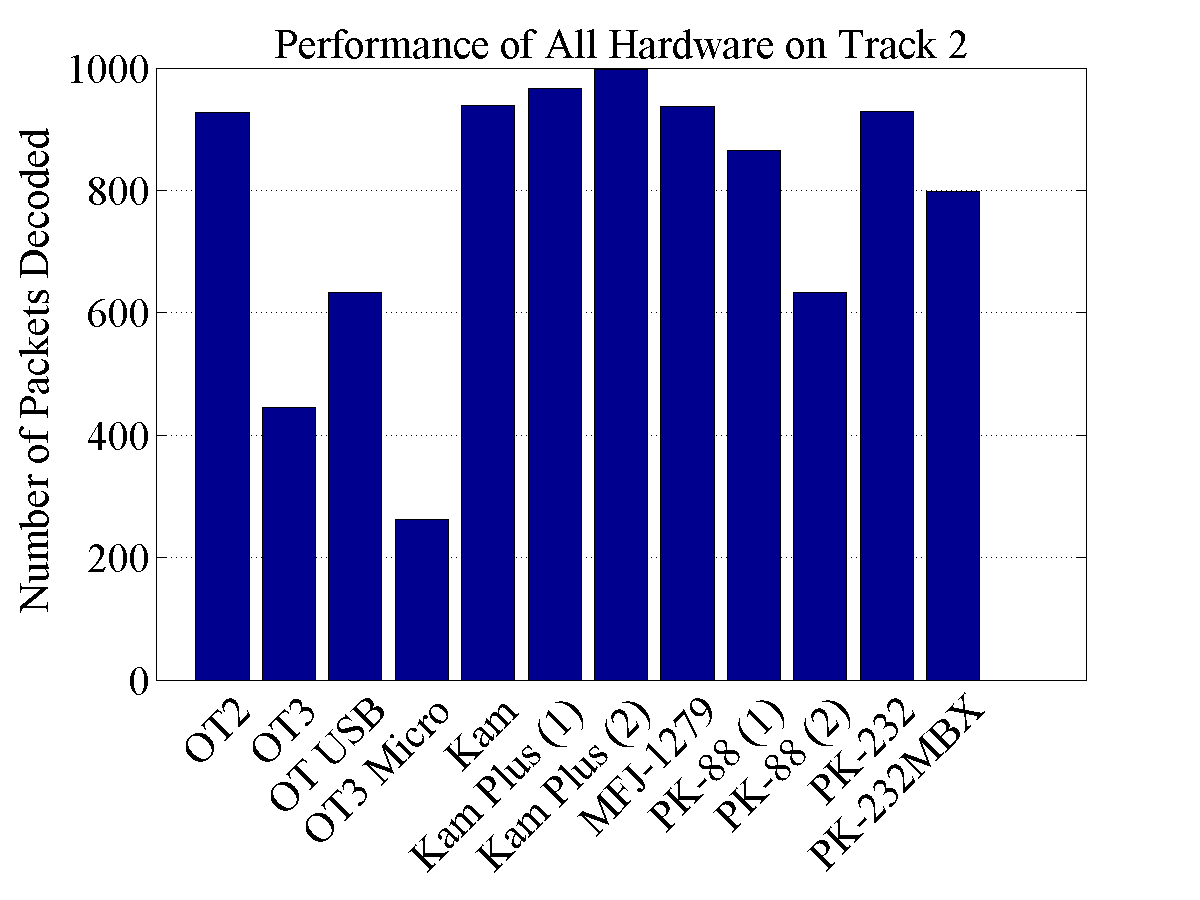
\includegraphics[width=0.75\linewidth]{images/PerformanceofAllHardwareonTrack2.png} 
	\caption{Number of packets successfully decoded for all tested hardware on Open Tracker 3 test file with noise.}
   \label{allHardwareTrack2}
\end{figure}

\section{Software Results}

\subsection{Hardware and Software Comparisons}

